\chapter{Statistical methods}\label{ch:stat}

In the course of analyzing the data sets provided by the CMS experiment and used in this thesis, several statistical tools have been employed; in this chapter, a description of these tools will be presented, starting with the general statement of the multivariate analysis method, followed by the particularities of the Boosted Decision Trees (BDT) method and its application to the classification problem. Statistical inference methods used will also be presented. This chapter is based mainly on the reference \cite{mva}.      

\section{Multivariate analysis}

Multivariate data analysis (MVA) makes reference to statistical techniques that analyze data containing information of more than one variable, commonly taking into account the effects of all variables on the response of the particular variable under investigation, \ie, considering all the correlations between variables. MVA is employed in a variety of fields like consumer and market research, quality control and process optimization. From a MVA it is possible to identify the dominant patterns in the data, like groups, outliers and trends, and determine to which group a set of values belong; in the particle physics context, MVA methods are used to perform the selection of certain type of events, from a large data set, using a potentially large number of measurable properties for each event.

Processes with small cross section, as the \tHq process, normally are hidden behind more common processes; therefore, the data set results in a subset of events with characteristic features of interest (signal) mixed in randomly with a much larger number of SM events that can mimic these features of interest (background) which implies that it is not possible to say with certainty that a given event is signal or background. In that sense, the problem can be formulated as one where a set of events have to be classified according to some features; these features correspond to the measurements of several parameters like energy, momentum organized in a set of ``input variables''. The measurements for each event can be written in a vector $\textbf{x}=(x_1,.....,x_n)$ for which

\begin{itemize}
\item Signal hypotheses $\to f(\textbf{x}|s)$ is the probability density (``likelihood'') for $\textbf{x}$ given it is a signal event 
\item Background hypotheses $ \to f(\textbf{x}|b)$ is the probability density (``likelihood'') of $\textbf{x}$ given it is a background event
\end{itemize}

Figure \ref{fig:scatter_plot} shows three ways to perform a classification of events for which measurements of two properties, two input variables, have been performed; blue circles represent signal events while red triangles represent background events. The classification on (a) is ``cut-based'' requiring $x_1<c_1$ and $x_2<c_2$; usually the cut values are chosen according to some knowledge about the event process. In (b), the classification is performed by stating a cut involving a linear function of the input variables and so the boundary, while in (c) the the relationship between the input variables is not linear thus the boundary is not linear either.          

\begin{figure}[!h]
  \centering
  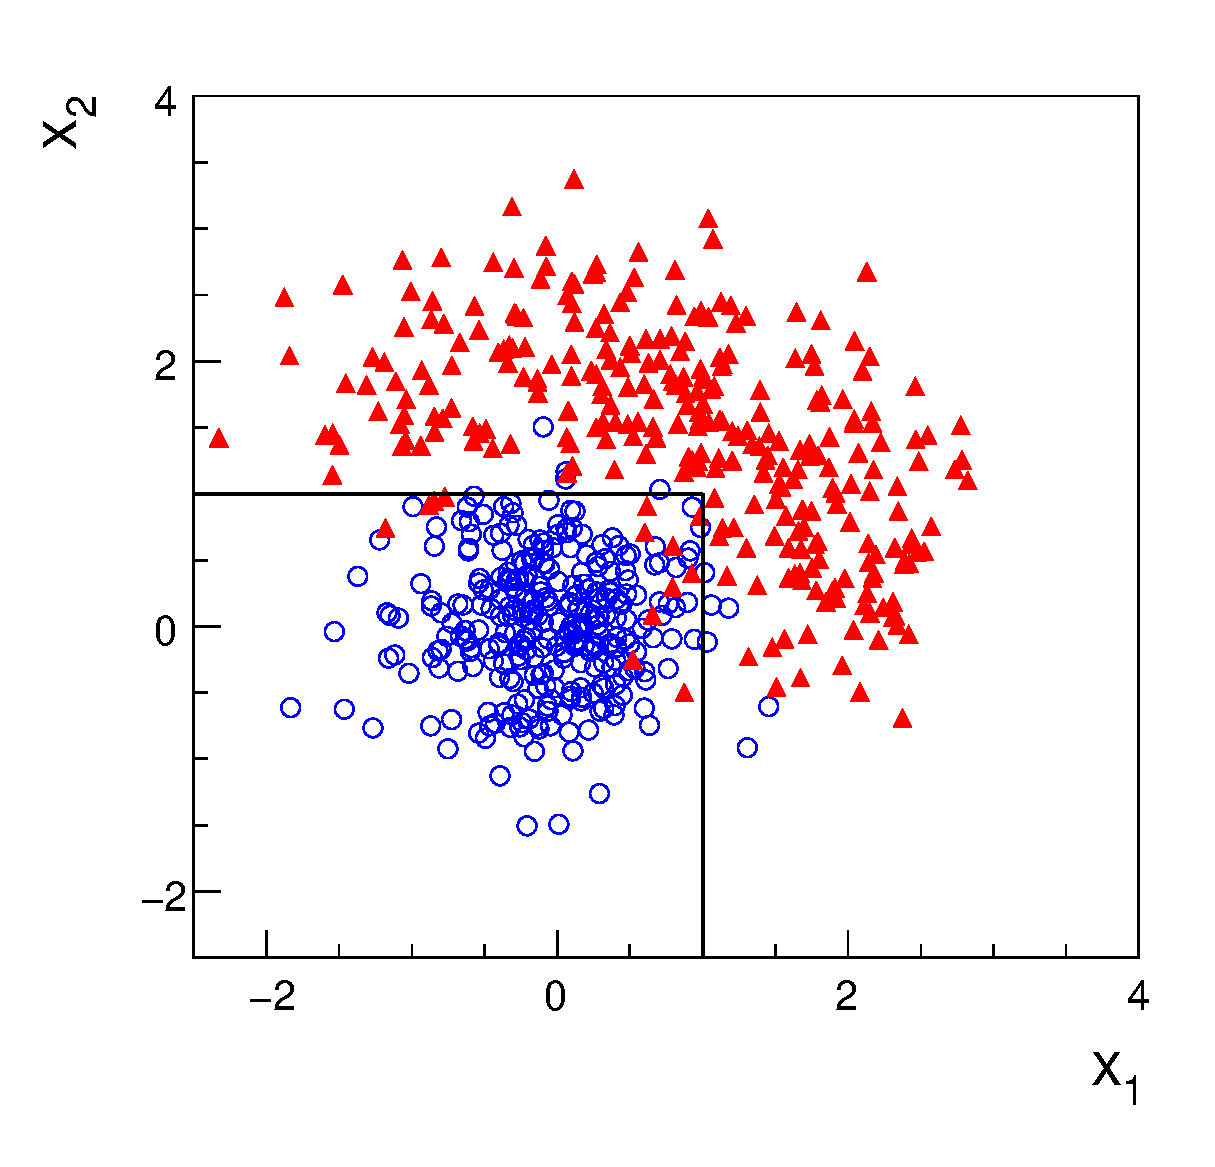
\includegraphics[width=4.5cm,height=4.5cm]{Cuts}
  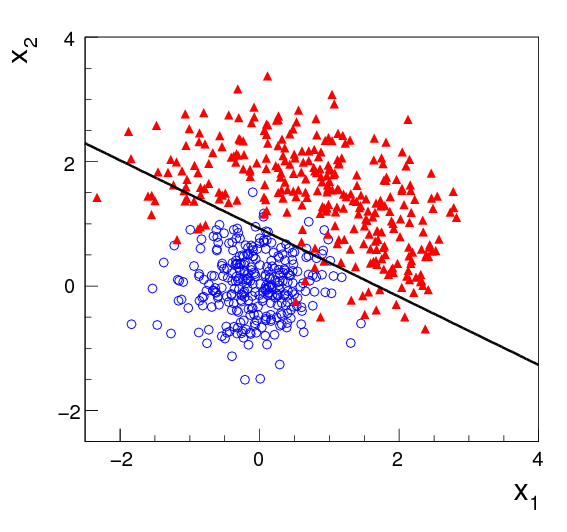
\includegraphics[width=4.5cm,height=4.5cm]{Fisher}
  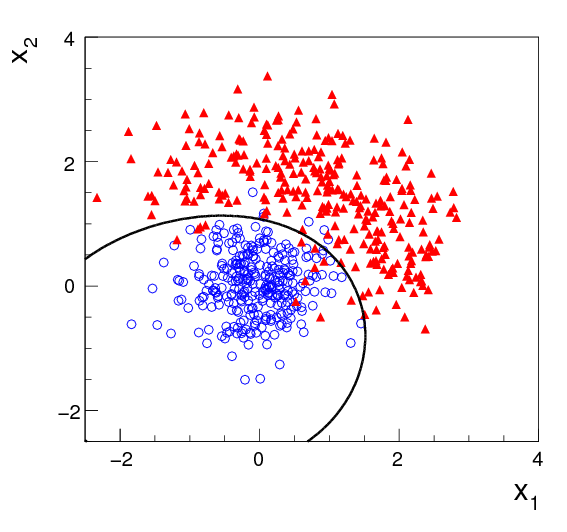
\includegraphics[width=4.5cm,height=4.5cm]{SVM05}
  \caption[Scatter plots-MVA event classification.]{Scatter plots-MVA event classification. Distribution of two input variables $x_1$ and $x_2$ measured for a set of events; blue circles represent signal events and red triangles represent background events. The classification is based on (a) cuts, (b) linear boundary, and (c) nonlinear boundary\cite{mva}}\label{fig:scatter_plot}
\end{figure}

The boundary can be parametrized in terms of the input variables such that the cut is set on the parametrization instead of on the variables, \ie, $y(\textbf{x})=y_{cut}$ with $y_{cut}$ a constant; thus, the acceptance or rejection of an event is based on what side of the boundary is the event located. If $y(\textbf{x})$ has functional form, it can be used to determine the probability distribution functions $p(y|s)$ and $p(y|b)$ and then perform a scalar test statistic with a single cut on the scalar variable $y$. 

\begin{figure}[!h]
  \centering
  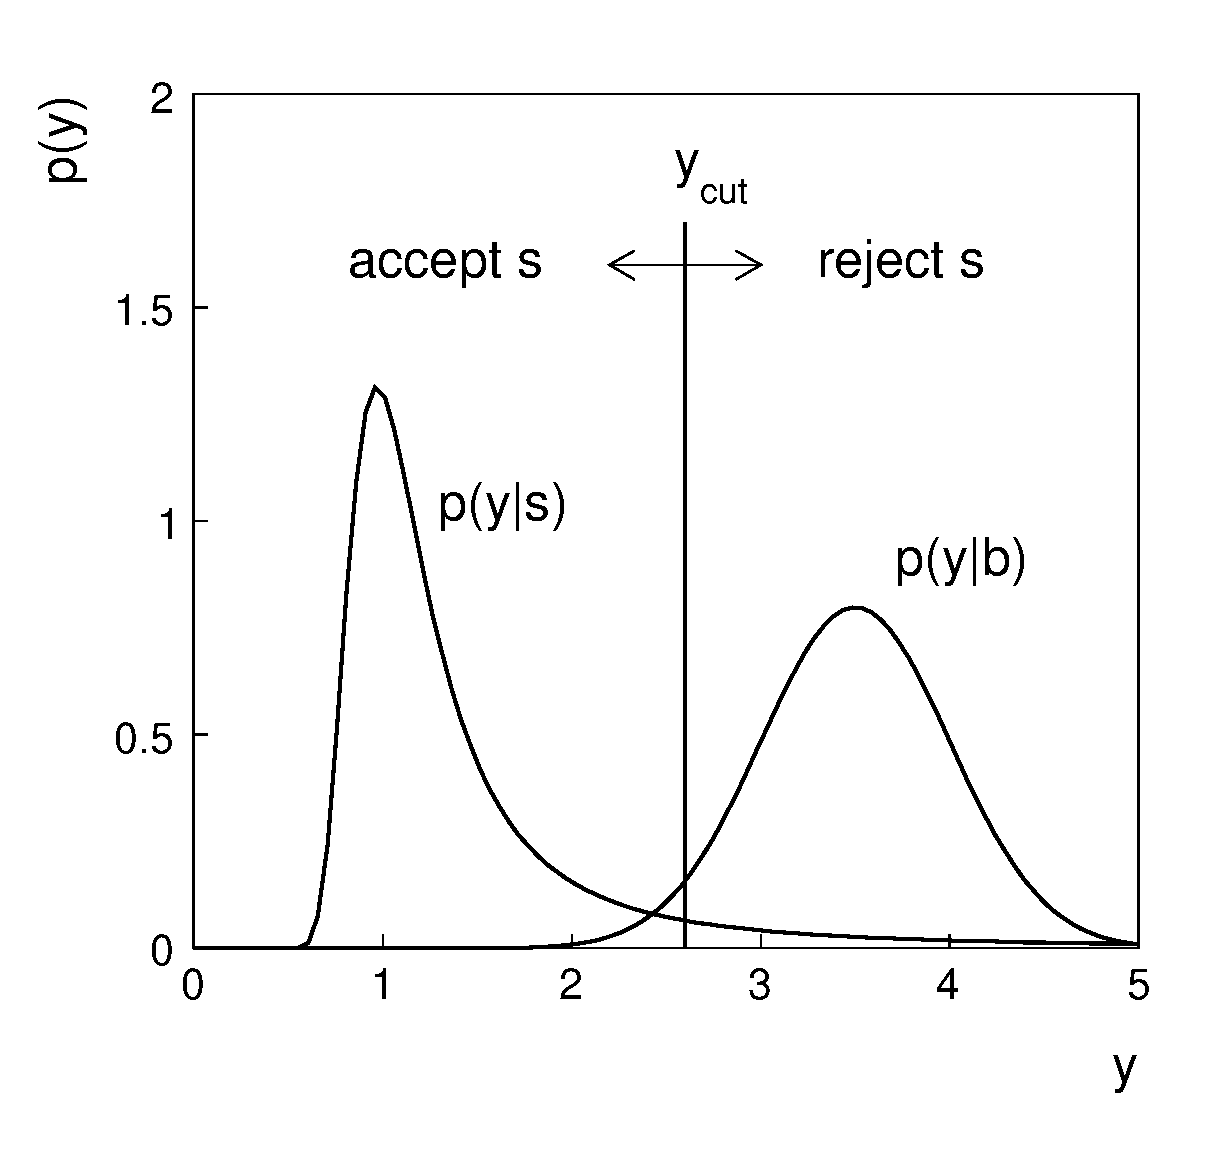
\includegraphics[scale=0.4]{TestStat}
  \caption[Scalar test statistical.]{Distributions of the scalar test statistic $y(\textbf{x})$ under the signal and background hypotheses.\cite{mva}}\label{fig:scalar_test}
\end{figure}

Figure \ref{fig:scalar_test} illustrates what would be the probability distribution functions under the signal and background hypotheses for a scalar test statistic with a cut on $y$.


\subsection{Decision trees }

For this thesis, the implementation of the MVA strategy, described above, is performed through decision trees. In a simple picture, a decision tree classifies events according to their input variables values by setting a cut on each input variable and checking which events are on which side of the cut, just as proposed in the MVA strategy, but in addition, as a machine learning algorithm, decision trees offer the possibility to be trained and then perform the classification efficiently.    

\begin{figure}[!h]
  \centering
  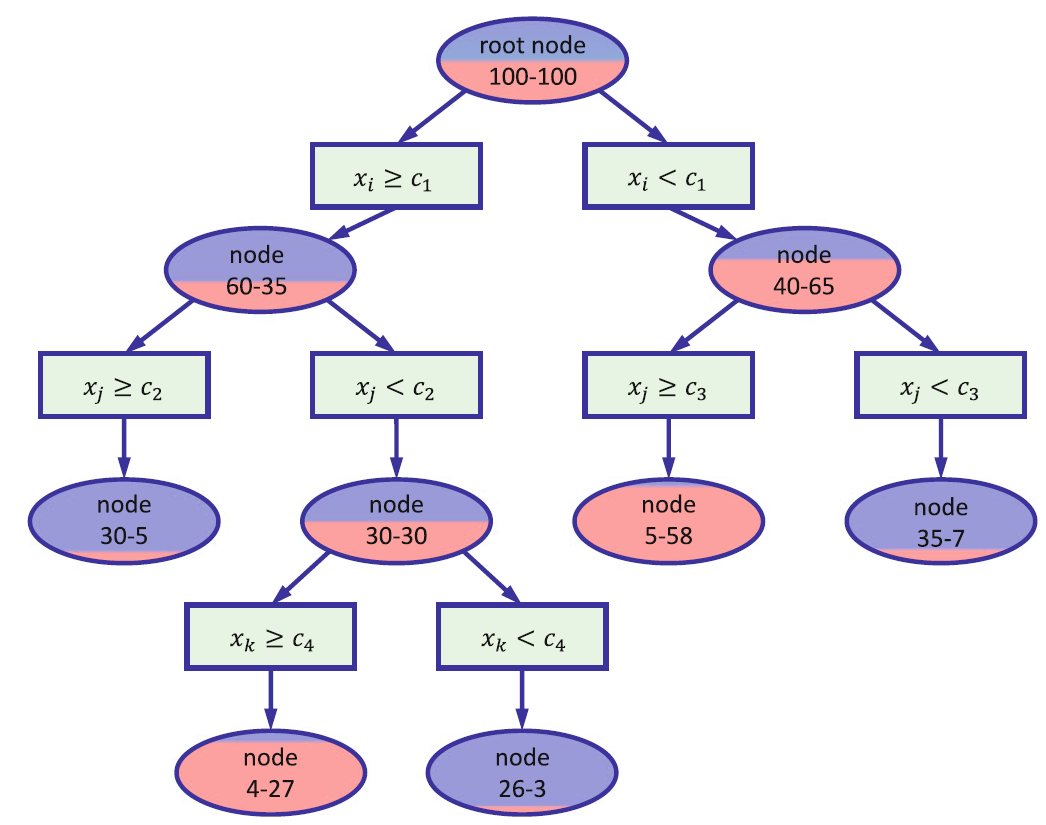
\includegraphics[scale=0.4]{decision_tree}
  \caption[Decision tree.]{Example of a decision tree. Each node is fed with a MC sample mixing signal and background events (left-right numbers); nodes colors represent the relative amount of signal/background events \cite{luca}.}\label{fig:dt}
\end{figure}

The training or growing of a decision tree is the process that defines the rules for classifying events; this process is represented in figure\ref{fig:dt} and consist of several steps

\begin{itemize}
\item take MC samples of signal and background events and split them into two parts each; first parts form the training sample which will be used in the decision tree training, while the second parts form the test sample which will be used for testing the final classifier obtained from the training. Each event has associated a set of input variables $\textbf{x}=(x_1,.....,x_n)$ which serve to distinguish between signal and background events. The training sample is taken in at the root ``node''. 
\item pick one variable, say $x_i$
\item pick one value of $x_i$, each event has its own value of $x_i$, and split the training sample into two subsamples $B_1$ and $B_2$; $B_1$ contains events for which $x_i< c_1$ while $B_2$ contains the rest of the training events;
\item scan all possible values of $x_i$ and find the splitting value that provides the ``best'' classification\footnote{ Quality of the classification will be treated in the next paragraph.}, \ie, $B_1$ is mostly made of signal events while $B_2$ is mostly made of background events.
\item It is possible that variables other than the picked one produce a better classification, hence, all the variables have to be evaluated. Pick the next variable, say $x_j$, and repeat the scan over its possible values.
\item At the end, all the variables and their values will have been scanned, the ``best'' variable and splitting value will have been identified, say $x_1, c_1$, and there will be two nodes fed with the subsamples $B_1$ and $B_2$. 
\end{itemize}

Nodes are further split by repeating the decision process until: a given number of final nodes is obtained, nodes are largely dominated by either signal or background events, or nodes has too few events to continue. Final nodes are called ``leaves'' and they are classified as signal or background leaves according to the class of the majority of events in them. Each ``branch'' in the tree corresponds to a sequence of cuts. 

The quality of the classification at each node is evaluated through a separation criteria; there are several of them but the ``Gini Index (G)'' is the one used in the decision trees trained for the analysis in this thesis. G is written in terms of the purity (P), \ie the fraction of signal events, of the samples after the separation is made; it is given by
\beqn
G=P(1-P)
\eeqn
\noindent notice that P=0.5 at the root node while G=0 for pure leaves. For a node $A$ split into two nodes $B_1$ and $B_2$ the G gain is
\beqn
\Delta G = G(A)- G(B_1)-G(B_2)
\eeqn

the `` best'' classification corresponds to that for which the gain of G is maximized; hence, the scanning over all event's variables and their values is of capital importance.

The output of a decision tree is called ``classifier''. Figure \ref{fig:dtr}

\begin{figure}[!h]
  \centering
  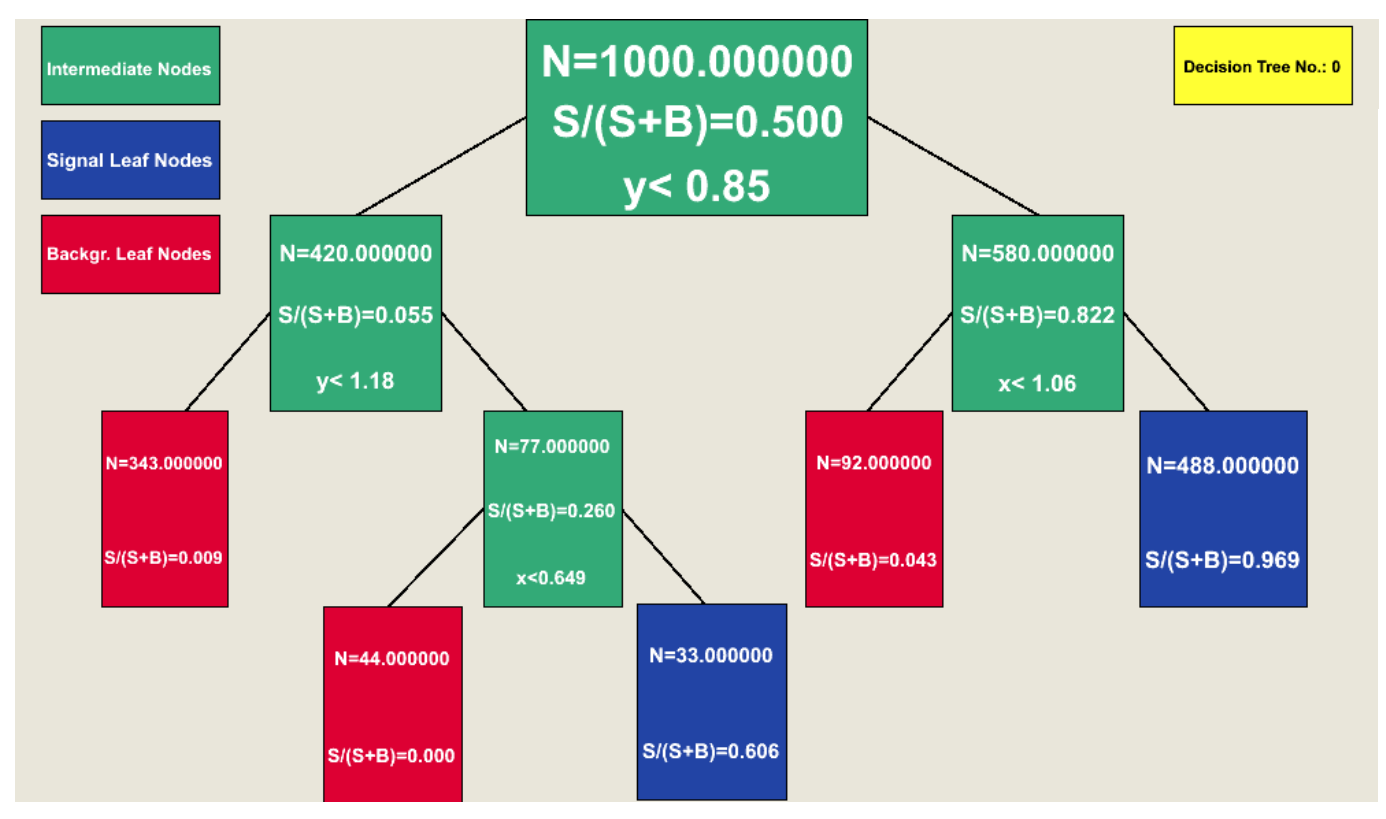
\includegraphics[scale=0.4]{dt1}
  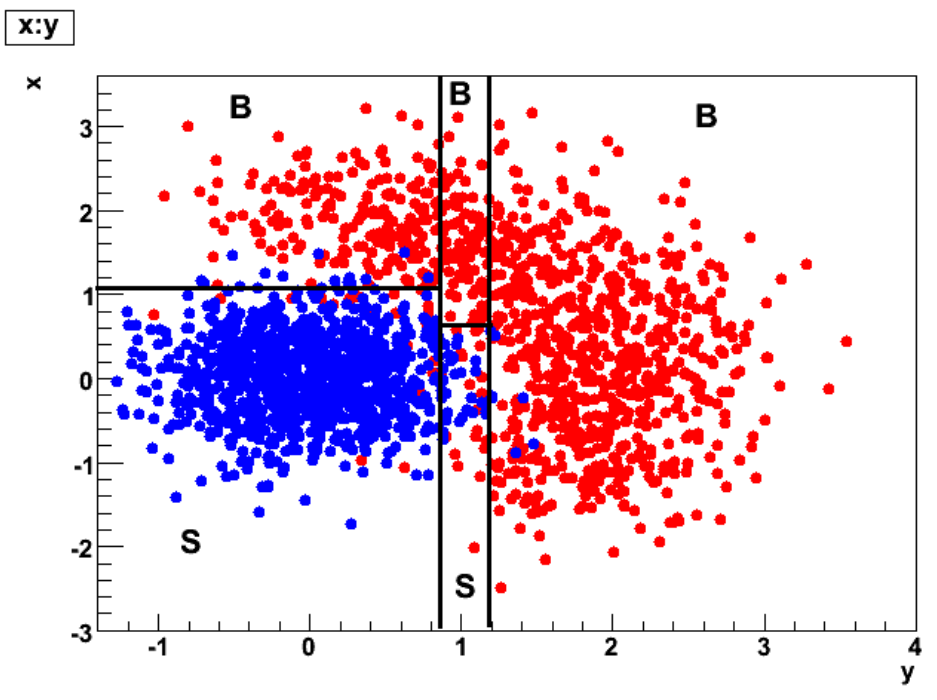
\includegraphics[scale=0.4]{dt2}
  \caption[Decision tree output example.]{Example of a decision tree output. Each leaf, blue for signal events and red for background events, represent a region in the variables phase space \cite{coadou}.}\label{fig:dtr}
\end{figure}

\subsection{Boosted decision trees (BDT)}

Event misclassification occurs when a training event end up in the wrong leaf, \ie, a signal event end up in a background leaf or a background event end up in a signal leaf; a way to correct it is to assign a weight to the misclassified events such that when used in the training of a new decision tree they get correctly classified. In the first decision tree all the weights are set to the unity, hence, an event with increased weight is a ``boosted'' event. The event reweighting if performed by a boosting algorithm which also creates a set of trees,  and hence a set of classifiers, which are combined to create a new classifier; this new classifier offers more stability and has a smaller misclassification rate than any individual ones.


It is often applied to decision trees, precisely because they suffer from sensitivity to statistical fluctuations in the training sample, but the technique can be applied to any classifier.



 






\beqn
P=\frac{\sum_s w_s}{\sum_s w_s + \sum_b w_b}
\eeqn

\noindent where $w_s$ and $w_b$ are the weights of the events in a weighted sample;  





%% where w i are the normalized weights for each event. The best possible question for the node
%% can then be determined by maximizing S,

By using a multitude of slightly altered decision trees and averaging over the predicted outcome
%% the robustness of the procedure can be ensured, as a badly trained tree due to aberrations does
%% not have enough power to sway the decision into the wrong direction. The average of all
%% classifier outputs is later used as a final discrimination variable, labeled as ”BDT output”.




 Notice that the tails of the distributions indicate that some signal events fall on the rejection region and some background events fall on the acceptance region; therefore, it is convenient to define the ``efficiency'' with which events of a given type are accepted, thus, the signal and background efficiencies are given by 

\begin{eqnarray}
\label{eq:sigeff}
\varepsilon_{\textrm{s}} & = & P( \mbox{accept event} | \mbox{s} ) = \int_{\textrm{A}} f(\textbf{x} | \mbox{s} ) \, d \textbf{x} = \int_{-\infty}^{y_{\textrm{cut}}} p(y | \mbox{s}) \, dy\;, \\*[0.3 cm]
\varepsilon_{\textrm{b}} & = & P( \mbox{accept event} | \mbox{b} ) = \int_{\textrm{A}} f(\textbf{x} | \mbox{b} ) \, d \textbf{x} = \int_{-\infty}^{y_{\textrm{cut}}} p(y | \mbox{b}) \, dy \;,
\end{eqnarray}

where A is the acceptance region. Under these conditions, the background hypothesis corresponds to the ``null hypothesis ($H_0$)'', the signal hypothesis corresponds to the ``alternative hypothesis ($H_1$)'', the background efficiency is the significance level of the test, and signal efficiency is the power of the test; what is sought in an analysis is to maximize the power of the test relative to the significance level.








; it is achieved, according to the Neyman-Pearson lemma\cite{npl},






by defining the acceptance region such that, for $\textbf{x}$ inside the region, the likelihood ratio, i.e., the ratio of probability distribution functions for signal and background,







\section{ MVA methods, NN, BDT, boosting, overtraining, variable ranking  }
\section{statistical inference, likelihood parametrization}
\section{ nuisance parameters}
\section{exclusion limits }
\section{asymptotic limits }


 









